\documentclass[10pt,a4paper,twocolumn]{article}
\usepackage{tm_styles}

\usepackage{subcaption}

% Package for floats[H] in Appendices
\usepackage{float}
\usepackage{verbatim}

%% Uncomment this lines for superscript citations instead
% \usepackage[super]{natbib}

%% Uncomment these lines for author-year citations instead
% \usepackage[round]{natbib}
% \let\cite\citep

\newcommand\wordcount{
    \immediate\write18{texcount -sub=section \jobname.tex  | grep "Section" | sed -e 's/+.*//' | sed -n \thesection p > 'count.txt'}
(\input{count.txt}words)}

\usepackage{url}
\usepackage{apacite}
\bibliographystyle{apacite}

\usepackage{nameref}
\usepackage[at]{easylist}
\usepackage{gensymb}

\graphicspath{ {imgs/} }


\makeatletter
\newcommand{\ei@aux}[1]{\begin{easylist}[itemize] #1 \end{easylist}\endgroup}
\newcommand{\ei}{\begingroup\Activate\ei@aux}
\makeatletter

\begin{document}

\title{\textit{Variational Bayesian Inference in Noisy Spiking Networks}}
\author{Berend Ottervanger, Kai Standvoss}

\maketitle
\thispagestyle{fancy}
\begin{abstract}


\end{abstract}
\section{Introduction}
\subsection{Bayesian Deep Learning}
Many Machine Learning tasks previously deemed far out of our reach have been solved, often beyond all prior expectations, with the advent of Deep Learning. \emph{Deep Learning} describes the use of a certain type of artificial neural networks --- rate based models that are arranged in layered, usually feed-forward architectures. Artificial neural networks take loose inspiration of the computational principles of the human brain (cite). Artificial \emph{neurons} constitute principal units of computation --- in practice they describe non-linear transformations of the hierarchical representations favored by the type of architectures used. 

Artificial neural networks are no new idea in artificial intelligence research. The original MacCulloch Pitts? unit dates back more than seventy years (cite) and since then many different approaches alongside the now prevailing Deep Learning systems have been developed (cite). The recent success of deep learning can be explained by its massive parallelizability on modern graphical computing units and the availability of enormous datasets that allow for efficient training of the often highly over parameterized models. Favored by rapid developments in both these prerequisites, Deep Learning has primarily addressed statistical pattern extraction tasks like image and speech recognition (cite).

A traditionally rather orthogonal approach in Machine Learning is given by Bayesian techniques. Here, close attention is given to the right level of model complexity and non-parametric models are used to tackle challenging, small data problems (cite). While Deep Learning systems often claim biological inspiration on Marr's algorithmic level of description (cite), Bayesians issue explanatory adequacy on  the computational level (cite). In fact a paradigm shift in neuroscience sees an increasing amount of explanations of cognitive phenomena and neural information processing using Bayesian models (cite).

Given that both approaches address different theoretical and practical problems in artificial intelligence and machine learning and might serve as useful characterizations of human cognition on different levels of description, naturally, early research has sought to conjoin both paradigms. Research in Bayesian Deep Learning (BDL) rose during earlier episodes of popularity of artificial neural networks but fell out of fashion together with the core field of Deep Learning during the second? ``AI Winter'' (cite). Now that Deep Learning systems have made their way into main stream applications the focus again has shifted towards marrying the well understood Bayesian techniques with these successful models. Bayesian Deep Learning promises several advantages over classical approaches. The use of adequate priors could allow for training large architectures even with relatively little available data, e.g. in the medical domain (cite). At the same time priors could be used to address the challenging problem of transfer learning between similar tasks (cite). Additionally, Bayesian techniques enable a principled way for model comparison --- a problem that currently is often addressed rather empirically. More generally, Bayesian models can make use of a long history of mathematically rigorous investigation. This could help overcome a frequent criticism of Deep Learning systems, that they act as mere \emph{black box} models that are not sufficiently understood to be of real scientific value (cite).
%%MAYBE also mention integration over unknown parameters!
Finally, Bayesian methods seek to compute posterior distributions over the quantities of interest such that more than single point estimates can be given as answers to a problem. While it is clear that giving an exact probability distribution over the posterior is intractable in general (cite), 
confidences or uncertainties in the estimated expected values can be provided.
BDL in this sense is a more rigorous approach to sampling from the posterior distribution as compared to classical DL. Whereas DL approaches get a single sample from the posterior distribution --- because they only sample from the prior distribution once, deterministically ---, BDL allows for getting a much clearer picture of the posterior, giving an approximate posterior distribution.
This feature offers a variety of advantages and is especially relevant in critical domains were model failure is costly and Machine Learning systems are meant to replace human oversight (cite). Moreover, a system's ability to critically reflect upon its own computations is highly relevant for research in artificial intelligence and cognitive science. 

\subsubsection{Relevance of Uncertainty}

A key property of Bayesian models is the availability of uncertainty estimates over the predicted quantities. In practice this means that Bayesian Deep Learning models output an expected value obtained through integration over all possible network weights and an uncertainty or precision estimate given by the variance of the estimated quantity. Whereas classical Deep Learning systems output only a softmax distribution for classification tasks or an individual point estimate in the case of regression, BDL thus offers additional information on the model's confidence in its prediction.

This information can be useful, for example, to detect out-of-data samples that could be classified with high softmax probability in one model, but in fact would have very high variance in the prediction of different models. Such out-of-data sample checks can be used to allow a human expert to step in, preventing possible failure. This is important whenever the result of a failure is potentially dramatic, for example in medicine or in (semi-)autonomous vehicles.

At this point it is relevant to distinguish between different kinds of uncertainty. Bayesian modelling differentiates between so-called \emph{alleatoric} uncertainty, which describes the irreducible uncertainty of the data, and \emph{epistemic} or model uncertainty, reflecting the uncertainty in an imperfect model of the data generation process \cite{kendall2017uncertainties}. All systems with imperfect sensors have to deal with the former kind of uncertainty and modelling it explicitly can be especially useful for weighting different input modalities. The latter kind of uncertainty can be decreased by gathering more data to improve the model of the world. Epistemic uncertainty is particularly interesing from a cognitive stance since it reflects the system's introspective ability to estimate the quality of its own models. 

Humans are certainly very good at estimating both kinds of uncertainty, but the ability to ``know what one does not know'', i.e. estimating epistemic uncertainty, truly distinguishes human cognition. Hence modelling this capacity seems key to any model of human cognition. Humans constantly seek to reduce epistemic uncertainty through active inference, a prominent example being saccadic gaze behavior \cite{mirza2018human}.
This way of maximizing information could equip computational models with the ability to actively seek new training data that is most relevant to improving itself. 

\subsubsection{Uncertainty as Relevance}
%Uncertainty may also lead to insight in the relevance of samples. If one sample is high in uncertainty, that might mean that the network has not yet learnt to deal with this kind of input.
The relvance problem is the problem of finding aspects of a problem that are relevant to solving it. Without spending too many resources sifting through the entire input. There could be a large portion of the input that is not at all relevant. That means that whenever an agent is not able to solve a problem with the knowledge it has, attending to parts of the input that it is not sure what to do with might be a good strategy.

To see why this is the case, let's take the famous example of Dennett's on the robot that tries to recover its battery. There is a room with a wagon in it, the robot's battery is on the wagon, but so is a time bomb. The problem is that the robot doesn't know what is relevant to getting the battery out (but not the bomb).
Here we assume that the robot has a model of the world, that is it has predictions about its future inputs. If the robot has any experience with rooms, it might expect the room not to do anything whatever it does. It might already have uncertainty about what would happen to the wagon when interacting with it, or it might learn that it doesn't react as expected when interacting with it. It could use this to adapt its expectations about how it can interact with it. Once it is clear how it can interact with the wagon, the same can be done for the battery. Uncertainty would thus be a guide to PULLOUT(Wagon, Room, t), PICKUP(Battery, t+1), PUSHIN(Wagon, Room, t+2), for example, safely extracting the battery from the room. 

One indicator of what is relavant are sources of maximal information gain, i.e. high uncertainty. Examples blalba.
alleatoric vs. epistemic uncertainty

\subsubsection{Monte Carlo Dropout}
%copied from proposal
Because of the large amounts of variables, deep neural networks are prone to overfitting (cite). Meaning they tend to learn a mapping of the specific input-output pairs in the dataset. This is detrimental as it generally means that the network gives very poor predictions for samples that the network was not trained on. So too in real-world cases, where non-experts may work with the system, expecting sensible outputs. Until 2012, to reduce overfitting behaviour in deep neural networks one had to train an ensemble of networks. This is slow because essentially one trains the same network multiple times, resulting in either long training or smaller networks. However \citeA{hinton2012improving} showed that stochastically dropping elements from the computation during training reduces overfitting. As the title of their paper says, it does so by ``preventing co-adaptation of feature detectors''. That is, feature detectors that only result in sensible activation patterns when certain others do (which depends on the specific sample), are selected against. This is because the feature detectors such a detector is dependent on might be randomly dropped out during training \cite{srivastava2014dropout}.

Dropout has since been given a probabilistic interpretation, as placing a Bernoulli prior over the network weights by \citeA{gal2016dropout}. This lets us view it as a Bayesian neural network that approximates Bayesian inference in a deep Gaussian process \cite{gal2016dropout}. Taking dropout networks to a Bayesian paradigm, they also introduce a method of obtaining uncertainty estimates from the network. This method they coined Monte Carlo dropout. It involves, not only dropping elements from the computation during training, but also at test time. The prediction is then taken to be the average, while the uncertainty is calculated by taking the sample variance, over a number of forward passes through the network.
% end copy
That is, we sample the prior over the network weights to get a sample of the posterior as the output.

\subsection{Spiking Neural Networks}
Classical Deep Learning systems represent artificial neurons as nodes adding their inputs and applying a point-wise differentiable non-linearity, thus producing a continuous real-valued output. Real neurons on the other hand encode their output in discrete, binary spikes. To justify the biological inspiration of the former ``rate-based'' neural networks, it is sometimes argued that a node in such a network represents the average firing \emph{rate} of a whole population of real neurons \cite{rolls1998neural}. 

Another approach, doing the discrete nature of real neurons more justice, models artificial neural networks with spiking network nodes. In these systems often more accurate neuron models are employed and learning rules inspired by neural plasticity mechanisms are implemented (cite?). Yet, this biological plausibility often comes at a cost --- much larger systems of spiking neurons have to be implemented, simulating more complicated neuron models is costly, and the spiking nature of the networks makes the system non-differentiable, in turn prohibiting the use of the successful Deep Learning techniques. 

As the goal of this work is to investigate the explanatory adequacy of neural networks and at the same time improve it by endowing systems with the inherently human capability of estimating uncertainties, we want to implement the aforementioned Bayesian techniques in more realistic spiking networks. 

To that goal, Nengo \cite{bekolay2014nengo} is used for the implementation of spiking versions of classical Deep Learning architectures. Nengo is a progaming framework that allows for simulation of large-scale neural networks of spiking and non-spiking neuron models, thereby helping to overcome the previously mentioned difficulties of spiking networks.

The Nengo extension NengoDL can run any kind of neural network implemented in Nengo using \emph{TensorFlow} \cite{abadi2016tensorflow} as the simulation backend. Thereby, neural networks can be efficiently run on a graphical processing unit. More specifically, Nengo offers continuous versions of the classical Leaky-Integrate-and-Fire (LIF) neuron. This neuron model can be used as a substitute activation function in classical Deep Learning architectures. These can then be trained in Nengo using standard gradient-descent optimization in continuous fashion. The relevant idea is, that during testing, the continuous activations, can be exchanged for the spiking version of the LIF neuron, effectively yielding a spiking implementation of the DL model \cite{hunsberger2015spiking}.

\subsubsection{Noise as a Resource}
The main research question of this work is, whether the inherent stochasticity of spiking networks can act in the same way as the randomized forward passes in Monte Carlo Dropout and thereby estimate uncertainty through approximate variational inference. 

Noise in biological systems and models thereof is often viewed as a nuisance or computational limitation, artifact of a biological substrate \cite{maass2014noise}. Yet, it is known from research in computational complexity, that randomized algorithms can efficiently solve many problems and often even provide the fastest available solution to a task \cite{motwani2010randomized}. More generally, the class of problems that is solvable by a probabilistic Turing machine \textbf{PP} contains \textbf{NP}, the famous class of ``difficult computational problems''. Even though problems in \textbf{PP} are considered intractable since the error probability of algorithms solving them cannot be bounded away from $\frac{1}{2}$ polynomially, this further highlights the computational virtues of randomization. 

In that light, research in neuroscience has come to except noise as a computational resource instead of an implementational burden \cite{maass2014noise}.

An alternative definition for PP, the complexity class of problems that a probabilistic Turing machine can solve in polynomial time, is the class of problems that a non-deterministic Turing machine solves in polynomial time, accepting only if a majority of the computation paths ends in an accepting state.
Explain noise as computational resource, relate to randomized algorithms and complexity classes

\subsubsection{Biological Systems}
explain energy efficiency

relevance for cognitive science
If spiking neural networks can, by giving them (approximately) the same input multiple times arrive at better predictions and uncertainty estimations, then biological neuronal networks can do the same. This would, in other words, be 

\subsection{Related Work}
explain primarly gals paper and why we do the same

\section{Methods}

In this work, classical Deep Learning architectures were trained using Nengo and then converted into spiking neural networks in order to investigate the effect of stochastic firing behavior as a mean of obtaining uncertainty estimates. Unlike real neural networks or spiking models thereof, DL models classically operate in a mere feed-forward fashion. That is to say that the input to the network is presented solely to a dedicated input layer which maps it to the next layer of the network through multiplication with a weight matrix, abstracting synaptic weight transmission. The subsequent layer applies a non-linear transformation to its input and passes its activation --- viewed as the firing rate of a population of cortical neurons  --- to the next layer of the network. This is done for several layers until a final output layer is reached were the output is compared to a desired target output during training or taken as the networks prediction for testing. The network is trained through gradient descent (cite) by backpropagating the error signal computed between the network output and the target. No feedback through horizontal of top-down projections is provided.

In Nengo, ensembles of artificial neurons constitute basic building blocks of computation. Nengo provides a variety of neuron models, whereof Leaky-Integrate-and-Fire (LIF) neurons (cite) were employed in this project. LIF neurons are very simplified models of neural computation, yet provide a sufficient level of complexity to our goals while being efficiently simulated. LIF neurons integrate their input until an individual firing threshold is reached and the neuron spikes, resetting its membrane potential back to a baseline value and not being able to spike again for a certain refractory period. Hence, LIF neurons are temporally dependent and spike stochastically in that their state does not merely depend on the input but also its past states and the background activity in the ensemble (injected by Nengo). This property is relevant to our research question, since it allows us to integrate the activity of the output layer of our network over several time steps and take the individual samples as samples of the posterior distribution learned by the network. 

An ensemble of neurons in Nengo seeks to cover its input domain uniformly by sampling an individual tuning curve for each of its neurons. The joint activation to an input signal given these different tuning curves allows to uniquely encode the input to the population.  

To train a DL model in Nengo network nodes in the DL architecture are substituted by Nengo's neuron ensembles of LIF units. Ensembles are connected by simulated synapses which can implement temporal delays and smoothing. Here, synapses are initialized to merely pass on the activation after multiplying it with its associated weight so to represent normal weights in a DL model. As mentioned, we exploited the efficiency of training through Backpropagation by substituting the LIF neurons by continuous versions thereof. These \emph{SoftLIF} units temporally smooth the neurons spikes, thereby encoding its instantaneous firing rate. Different network architectures were used for the experiments described in the following section. All models were trained with classical dropout, performing approximate variational inference according to \cite{gal2016dropout}.

During testing of the trained models, the SoftLIF units were exchanged for their spiking counterparts while maintaining the rest of the network architecture. In order to simulate dropout in classical networks, each test input was presented to the network for an extended period of time while propagating the activity through the network. The spiking behavior of the LIF neurons naturally simulates the random deactivation of neurons using dropout. Therefore, the network output varies over time. Collecting this output for a number of time steps $T$ allows to obtain a mean activation and its variance, representing the models epistemic uncertainty. If the model is trained extensively the network output should vary relatively little, corresponding to very confident predictions, while an untrained model will oscillate strongly. 

In order to test the suitability of the described approach to obtain uncertainty estimates, both the classical MC dropout with rate based neurons as well as the spiking version were applied to the same test data. The results were analyzed both quantitatively as well as qualitatively. For qualitative analysis, the mean network outputs are visualized alongside the networks uncertainty estimate. Quantitatively, the uncertainty estimate obtained by MC dropout is taken as a reference standard and correlated with the uncertainty estimates from the trained spiking network and a non-trained baseline architecture. Mean and standard deviations of 10 simulations are reported in the results section.   

\section{Experiments}
Two different experiments were performed to investigate the suitability of our proposed technique. Both experiments were taken from the original literature proposing the use of dropout to obtain Bayesian uncertainty estimates. The first experiment was introduced in a prominent Blogpost by Yarin Gal (cite) and constitutes a toy example that allowed for comparison on a simple task. The second experiment is taken from \cite{gal2016dropout} introduced to motivate the suitability of MC dropout for obtaining uncertainty estimates. Both experiments deal with regression tasks. 

\paragraph{Experiment I} In the first experiment a neural network is trained to approximate a simple one-dimensional function:

\begin{align}
f: \mathds{R} \to \matds{R}, x \mapsto x\sin{(x)}
\end{align}

visualized in Figure \ref{fig:exp1_func}.

\begin{figure}
\centering
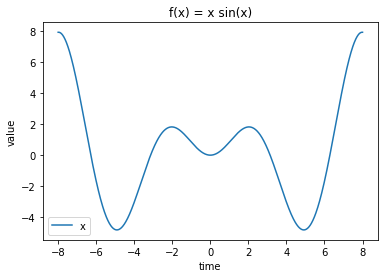
\includegraphics[]{function.png}
\caption{Visualization of the function f learned in Experiment I}\label{fig:exp1_func}
\end{figure}
\section{Results}

\section{Discussion}

\bibliography{sources}

\end{document}